\documentclass[acmsmall, anonymous, review, screen]{acmart}

\usepackage{syntax}
\usepackage{booktabs} % For formal tables
\usepackage{mathtools}
\usepackage{forest}
\usepackage{subcaption}
\usepackage[ruled]{algorithm2e} % For algorithms

\usepackage{tikz}
\renewcommand{\algorithmcfname}{ALGORITHM}
\SetAlFnt{\small}
\SetAlCapFnt{\small}
\SetAlCapNameFnt{\small}
\SetAlCapHSkip{0pt}
\IncMargin{-\parindent}


% Metadata Information
%\acmJournal{TWEB}
%\acmVolume{9}
%\acmNumber{4}
%\acmArticle{39}
%\acmYear{2010}
%\acmMonth{3}
%\copyrightyear{2009}
%\acmArticleSeq{9}

% Copyright
%\setcopyright{acmcopyright}
%\setcopyright{acmlicensed}
%\setcopyright{rightsretained}
%\setcopyright{usgov}
%\setcopyright{usgovmixed}
%\setcopyright{cagov}
%\setcopyright{cagovmixed}

% DOI
%\acmDOI{0000001.0000001}

% Paper history
%\received{February 2007}
%\received[revised]{March 2009}
%\received[accepted]{June 2009}

\usepackage{xcolor}
\newcommand\todo[1]{\textcolor{red}{#1}}

% Document starts
\begin{document}
% Title portion. Note the short title for running heads 
\title[Spineless]{Spineless Traversal for Layout Invalidation}  
\author{Marisa Kirisame}
\email{marisa@cs.utah.edu}
\orcid{1234-5678-9012-3456}
\affiliation{%
  \institution{University of Utah}
  \streetaddress{201 Presidents' Cir, Salt Lake City, UT 84112}
  \city{Salt Lake City}
  \state{UT}
  \postcode{84112}
  \country{USA}}
\author{Tiezhi Wang {2152591@tongji.edu.cn}}
\orcid{1234-5678-9012-3456}
\affiliation{%
  \institution{Tongji University}
  \streetaddress{104 Jamestown Rd}
  \city{Williamsburg}
  \state{VA}
  \postcode{23185}
  \country{China}}
\author{Pavel Panchekha {pavpan@cs.utah.edu}}
  \orcid{1234-5678-9012-3456}
  \affiliation{%
  \institution{University of Utah}
  \streetaddress{201 Presidents' Cir, Salt Lake City, UT 84112}
  \city{Salt Lake City}
  \state{UT}
  \postcode{84112}
  \country{USA}}

\begin{abstract}
Latency is a major concern for web rendering engines
  like those in Chrome, Safari, and Firefox.
These engines reduce latency by using
  an \emph{incremental layout algorithm}
  to redraw the page when
  the user interacts with it.
In such an algorithm,
  nodes that change frame-to-frame are marked dirty;
  only the dirty nodes need be processed
  to draw the next frame,
  dramatically reducing latency.
However, the standard incremental layout algorithm
  must search the tree for dirty nodes,
  accessing a number of auxiliary nodes
  in the process.
These auxiliary nodes
  add cache misses and stalled cycles,
  and are responsible for a sizable fraction
  of all layout latency.

We introduce a new, faster incremental layout algorithm
  called Spineless Traversal.
Spineless Traversal
  uses a more computationally demanding
  priority queue algorithm
  to avoid the need to access auxiliary nodes
  and thus reduces cache traffic and stalls.
This leads to dramatic speedups
  on the most latency-critical interactions
  such as hovering, typing, or animations.
Moreover, thanks to numerous low-level optimizations,
  we are able to make Spineless Traversal
  competitive across the whole spectrum of
  incremental layout workloads.
As a result, across on \NumFrames~benchmarks,
  Spineless Traversal is faster on \PctFaster,
  with a mean speedup of \MeanSpeedup,
  with the speedups concentrated in
  the most latency-critical interactions
  such as hovering, typing, or animations.
\end{abstract}

\newcommand{\DBPQoverheadCount}{2216}
\newcommand{\DBPQoverheadpctslowdown}{21.8\%}
\newcommand{\DBPQoverheadpctspeedup}{78.2\%}
\newcommand{\DBPQoverhead}{\ensuremath{3.23\times}\xspace}
\newcommand{\DBPQeval}{0.99}
\newcommand{\DBPQtotal}{\ensuremath{1.78\times}\xspace}
\newcommand{\DBPQsmalloverheadCount}{1346}
\newcommand{\DBPQsmalleval}{0.99}
\newcommand{\DBPQsmalltotal}{\ensuremath{2.35\times}\xspace}
\newcommand{\DBPQlargeoverhead}{1.29}
\newcommand{\DBPQlargeeval}{0.99}
\newcommand{\DBPQlargetotal}{1.17}
\newcommand{\TotalDiffCount}{2216\xspace}
\newcommand{\TotalTraceCount}{50\xspace}

\newcommand{\NumWebsites}{\TotalTraceCount}
\newcommand{\NumFrames}{\TotalDiffCount}
\newcommand{\MeanSpeedup}{\DBPQtotal}
\newcommand{\MeanSpeedupSmall}{\DBPQsmalltotal}
\newcommand{\PctSlower}{25.14\%\xspace}
\newcommand{\PctFaster}{74.86\%\xspace}
\newcommand{\PctSmall}{60.7\%\xspace}


%
% The code below should be generated by the tool at
% http://dl.acm.org/ccs.cfm
% Please copy and paste the code instead of the example below. 
%
\begin{CCSXML}
<ccs2012>
 <concept>
  <concept_id>10010520.10010553.10010562</concept_id>
  <concept_desc>Computer systems organization~Embedded systems</concept_desc>
  <concept_significance>500</concept_significance>
 </concept>
 <concept>
  <concept_id>10010520.10010575.10010755</concept_id>
  <concept_desc>Computer systems organization~Redundancy</concept_desc>
  <concept_significance>300</concept_significance>
 </concept>
 <concept>
  <concept_id>10010520.10010553.10010554</concept_id>
  <concept_desc>Computer systems organization~Robotics</concept_desc>
  <concept_significance>100</concept_significance>
 </concept>
 <concept>
  <concept_id>10003033.10003083.10003095</concept_id>
  <concept_desc>Networks~Network reliability</concept_desc>
  <concept_significance>100</concept_significance>
 </concept>
</ccs2012>  
\end{CCSXML}

\ccsdesc[500]{Computer systems organization~Embedded systems}
\ccsdesc[300]{Computer systems organization~Redundancy}
\ccsdesc{Computer systems organization~Robotics}
\ccsdesc[100]{Networks~Network reliability}

%
% End generated code
%

% We no longer use \terms command
%\terms{Design, Algorithms, Performance}

\keywords{Web Browser, Incremental Computation, Algorithms, Performance}


\thanks{This work is supported by the National Science Foundation,
  under grant CNS-0435060, grant CCR-0325197 and grant EN-CS-0329609.

  Author's addresses: G. Zhou, Computer Science Department, College of
  William and Mary; Y. Wu {and} J. A. Stankovic, Computer Science
  Department, University of Virginia; T. Yan, Eaton Innovation Center;
  T. He, Computer Science Department, University of Minnesota; C.
  Huang, Google; T. F. Abdelzaher, (Current address) NASA Ames
  Research Center, Moffett Field, California 94035.}


\maketitle

% The default list of authors is too long for headers}
\renewcommand{\shortauthors}{M. Kirisame et al.}
\section{Introduction}

Latency is a major concern for modern web rendering engines.
A rendering engine, such as that in Chrome, Firefox, or Safari,
  must redraw pages 60 times per second
  to guarantee smooth animations, fluid interactions,
  and responsive web applications.
When this frame rate cannot be met,
  the user experiences lag and may be forced to use another web application, browser, or device.
Modern 120\,Hz displays demand even lower latency.

Layout is a key driver of web rendering latency.
Layout means calculating the size and position
  of each element on the web page,
  after which the page can be rendered as pixels on the screen.
Every time the user interacts with the web page
  by hovering over an element,
  receiving updated data,
  or even observing an animation,
  the web page changes
   and must be re-laid-out.
Since layout is only one part of the larger rendering pipeline,
  this re-layout must be completed in a millisecond or less
  in order to meet the 60 frame-per-second goal.
On such a tight budget, every cycle counts!

\paragraph{Incrementalization}
The key optimization that makes this possible
  is \emph{incrementalization}.
When an element on the page changes,
  the browser \emph{marks} it dirty.
When the page is re-laid-out,
  the rendering engine traverses the page
  to find and re-lay-out only the dirty elements.
That might mark additional elements dirty,
  due to dependencies between elements,
  but typically---in, say, animations---%
  only a few nodes are ultimately re-laid-out.
In these cases, searching the tree
  for dirty elements is the bottleneck,
  especially since every element access
  is likely to incur a cache miss.

Browsers use the ``Double Dirty Bit'' algorithm
  to find dirty nodes more quickly~\cite{wbe,tali-garseil}.
This algorithm adds summary bits
  to identify and skip subtrees without any dirty elements.
While this reduces the search time,
  Double Dirty Bit still has to traverse the tree,
  starting from the root, to find dirty elements,
  and thus accesses not only the actually-dirty elements
  but many extra ``auxiliary nodes''.
On large pages,
  auxiliary nodes can significantly outnumber
  the actually-dirty elements;
  and since each node access can cause a cache miss,
  simply traversing these auxiliary nodes,
  just to check their summary bits,
  can stall the layout algorithm for hundreds of microseconds.
This problem is widely observed in practice;
  Google's widely-used web performance tool, Lighthouse,
  measures tree depth and maximum children count
  precisely because these parameters
  determine the number of auxiliary nodes.

\paragraph{Spineless Traversal}

We introduce \textit{Spineless Traversal}:
  a new, faster algorithm for incremental layout.
Unlike Double Dirty Bit,
  Spineless Traversal accesses only dirty elements,
  not auxiliary nodes.
It therefore reduces cache misses.
Spineless Traversal works by
  storing the set of dirty elements in a queue
  and jumping directly from one to the next,
  with no auxiliary nodes in between.

The key challenge is traversing the dirty nodes in the correct order. 
Recomputing a field on one node
  can mark fields on other nodes dirty,
  and the set of transitive dependencies is complex.
Fields must therefore be recomputed in a specific order,
  and Spineless Traversal must respect that order
  as it jumps from node to node.
Spineless Traversal thus stores
  a timestamp on each node,
  and uses a priority queue to traverse nodes
  in timestamp order.
To maintain timestamps as nodes are added and removed,
  Spineless Traversal \emph{order maintenance},
  which compute relative timestamps in a flexible way.
Both the priority queue and order maintenance structure
  are heavily optimized to make them competitive with Double Dirty Bit.

\paragraph{Implementation}

We implement Spineless Traversal in Megatron,
  a new compiler for incremental layout algorithms.
Megatron implements decades of research on attribute grammars:
  it statically analyzes the dependency graph,
  synthesizes recomputation and marking functions,
  and guarantees a correct incremental layout.
It implements standard optimizations
  (unboxing, interning, field packing, and jump tables)
  and compiles layout algorithms to highly efficient C++ code.
Megatron supports both Double Dirty Bit and Spineless Traversal
  via a common invalidation traversal interface,
  allowing an apples-to-apples comparison between them.

We compare the two algorithms on
  a significant fragment of web layout that includes
  line breaking, flex-box, intrinsic sizes, and many other features,
  benchmarking \TotalTraceCount real-world web pages
  like Twitter, Discord, Github, and Lichess.
Across \TotalDiffCount frames,
  Spineless Traversal is \DBPQtotal times faster on average.
Speedups are concentrated in the most latency-critical frames:
  on the \PctSmall of frames
  where at most 1\% of fields are recomputed,
  Spineless Traversal achieves a speedup
  of \MeanSpeedupSmall.


\section{Web layout}

Web pages are written in HTML,
  which is a tree-structured markup language
  containing text and elements that wrap it.
The web browser's parsed representation of this tree
  is called the DOM or HTML tree.
To draw the page to the screen,
  the browser applies a sequence of transformations---%
  called rendering phases---%
  to this DOM tree: matching, styling, layout, paint, and so on.
The focus of this paper, the layout phase,
  applies to an intermediate tree structure
  called a ``layout tree'',
  whose shape largely matches the DOM tree
  (though with some deviations for ``generated content''
  like bullets for list items).
The layout phase reads layout node properties
  (which reflect HTML attributes, CSS properties, and other data)
  and computes layout fields like width and height for those nodes.
Later phases like painting then read those layout fields
  and use them to draw the page to the screen.
The DOM and layout trees are typically poorly-balanced,
  with both lots of ``wrapper'' elements (with a single child)
  and also many ``list'' elements with many children;
  an example DOM tree for a small web page
  is shown in Figure~\ref{fig:dom-tree-db}.
In memory,
  the layout tree is stored as a pointer tree,
  with the children stored as a doubly linked list,
  to allow for fast insertions and deletions.
This pointer-heavy structure means
  that layout nodes are spread throughout memory,
  with every access typically generating a cache miss.

\subsection{The Layout Phase}

The layout phase computes a number of layout fields
  for each node in the layout tree.
Computing layout fields is a recursive process
  because each node's layout depends on the layout of its neighbors.
For example, the height of a node is (typically)
  the sum of the heights of all its children,
  while a node's $x$ position depends on the $x$ position
  of its previous sibling, plus that previous sibling's width.%
\footnote{
  In reality, these rules are quite a bit more complex,
    with various exceptions to the simplified sketch given here.
}
Moreover, visible properties like width and height
  in turn depend on intermediate properties such as intrinsic size,
  current line ascent/descent, and even more obscure properties
  like the sum of its siblings' \texttt{flex-grow} values.
A complete layout phase must visit each node multiple times,
  in a well-defined order,
  in order to compute each field on each node
  before any others that depend on it.

\begin{figure}
\begin{minipage}[b]{0.68\linewidth}
\begin{verbatim}
# real web layout much more complex
def layout_simple(self): 
  self.width <-
    if parent? then max(0, parent.width - 10)
    else 50 # screen size
  children.forEach(layout_simple)
  self.height <-
    if last? then last.height_acc + 10 # padding
    else self.attribute[height]
  self.height_acc <-
    if prev?
    then prev.height_acc + self.height + 10 # margin
    else self.height
\end{verbatim}
\caption{A layout algorithm that computes width and height of each dom node. The above program is a tree traversal: it walks down the tree then walks up the tree, computing values for each node during the walk.}
\label{fig:layout-simple}
\end{minipage}\hfill%
\begin{minipage}[b]{0.28\linewidth}
\centering
\includegraphics[scale=0.23]{LayoutExample.png}
\caption{The layout algorithm running on a layout tree of size 4. All nodes have an height attribute of 10.}
\end{minipage}
\end{figure}

We remark on a couple of key properties of layout
  that influence our approach:
\begin{enumerate}
\item Bounded work per node. There are no
  data-dependent loops, recursions, or data structures
  except the layout tree itself.
\item Immutable shape. The layout tree's structure
  is not modified during layout;
  only the layout fields on each node are.
Moreover, these computed fields
  are only written once (per frame)
  and then become read-only (for that frame).
\item Static control flow.
  The fields are computed in a fixed order
    dependent only on the layout tree shape,
    not the values of other computed fields.
\item Local data flow.
  To compute a particular node's fields,
    only that node's neighbors in the layout tree
    and their fields are accessed.
\end{enumerate}
These properties are discussed in
  the wealth of prior work on formalizing layout%
  ~\cite{meyerovich-1,meyerovich-2,meyerovich-3,cassius-1,cassius-2,cassius-3,yufeng-1,yufeng-2}.

In other words, layout can be expressed in the DSL
  shown in Figure~\ref{fig:dsl}, which is essentially an Attribute Grammar with the evaluation order scheduled and fixed.
In this DSL, a layout is defined by a set of passes
  $\text{Pass}_n$ performed in a certain order (the schedule).
Each pass performs a recursive, in-order traversal of the tree,
  computing some fields pre-order and some fields post-order.
Each field computation is a simple assignment $\mathsf{self}.V \gets T$,
  where $V$ is a field of the current node $\mathsf{self}$
  and $T$ is an expression that can refer to
  fields of $\mathsf{self}$ or its neighbors
  $\mathsf{parent}$, $\mathsf{prev}$, $\mathsf{next}$,
  $\mathsf{first}$ child, and $\mathsf{last}$ child.
Computations can also refer to HTML attributes or CSS properties
  of the current node
  using $\mathsf{attribute}[x]$ or $\mathsf{property}[x]$.%
\footnote{
We use two different namespaces
  for HTML attributes and CSS properties
  because some names, like \texttt{height},
  appear in both sets.
There is no other semantic difference between them,
  and other accessible properties,
  such as the tag name or image width and height
  do not affect invalidation traversal
  (but are modeled in our system as special properties).
}
Expressions can also use conditionals
  to test whether a given neighbor exists ($\mathsf{N?}$).
Notably, our DSL enforces
  the key properties of layout described above:
  there is no functionality to mutate the tree shape
  or to reorder control flow according to field values.
There are also no loops or data structures,
  and the only field access allowed is to a node's neighbors.

Many compound operations can be compiled into this DSL;
  for example, to access $\mathsf{parent}.\mathsf{parent}.\mathsf{x}$,
  one can instead define
  $\mathsf{self}.\mathsf{parent\_x} \gets \mathsf{parent}.x$
  to store each node's parent's $x$ field.
Then $\mathsf{parent}.\mathsf{parent}.x$
  is simply $\mathsf{parent}.\mathsf{parent\_x}$.
In any case, prior work in similar DSLs%
  ~\cite{meyerovich-1, meyerovich-2, cassius-1,
  cassius-2, cassius-3, yufeng-1, yufeng-2}
  has already shown that layout features
  like the CSS box model, intrinsic widths,
  absolute positioning, flexible box layout,
  and line breaking are expressible in this DSL.

\paragraph{Trace}
\label{par:trace}
A key property of a layout $L$
  is the order in which it computes
  different fields on different nodes in the tree.
Specifically, let the \emph{trace} of a layout on a tree $T$
  be sequence of $(n, v)$ pairs
  where $n$ is a node in $T$ and $v$ is a field name in $L$.
Because our DSL only performs in-order traversals,
  the trace is structurally related to the tree shape:
  local changes to the tree (node insertions or deletions)
  imply a local change to the trace (subtrace insertion or deletion).
This structural relationship means that the ordering of any two $(n, v)$ pairs is fixed:
If $(n, v)$ appears before $(n', v')$,
  this appear-before relationship will be maintained even as new nodes are added or removed.% 
\footnote{
  We assume here that
    only brand-new nodes, not previously-removed ones,
    are inserted into the tree.
  To our knowledge, this is true of all major web rendering engines.
}


In the remainder of this paper,
  we will assume a correct implementation
  of web page layout exists in this DSL,
  with correctness meaning both the correct set of rules
  that compute the fields required
  in the CSS standard~\cite{css}
  and also a correct schedule for computing those fields
  while preserving dependencies.
Our own implementation (Section~\ref{sec:layout-impl})
  implements a subset of CSS covering a variety
  of complex and widely-used web layout features;
  however, spineless traversal is applicable
  to any layout expressed in this DSL,
  and we do not focus on the details
  of the rules or schedule further.
Moreover, while this paper focuses on web layout,
  we expect spineless traversal to be applicable
  to a number of other incremental computations,
  differential dataflow, or semi-naive evaluation problems.

\begin{figure}

\begin{align*}
\text{Layout} &\coloneq  \text{Rule}^+; \textbf{schedule}\:\text{Pass}_n^+ \\
\text{Rule} &\coloneq
  \mathbf{def}\:\text{Pass}_n()\:\{\:
    A^+;\:
    \mathsf{children}.\mathsf{forEach}(\text{Pass}_n);\:
    A^+;\:
  \} \\
A \in \text{Assignment} &\coloneq
  \text{self}.V \leftarrow T \\[4pt]
T \in \text{Term} &\coloneq
  \text{if}\ T\ \text{then}\ T\ \text{else}\ T \mid
  F(T^+) \mid
  N? \mid
  N.V \mid
  \mathsf{attribute}[V] \mid
  \mathsf{property}[V] \\
N \in \text{Neighbor} &\coloneq
  \mathsf{self} \mid \mathsf{prev} \mid
  \mathsf{next} \mid \mathsf{parent} \mid
  \mathsf{first} \mid \mathsf{last} \\[4pt]
V \in \text{Variable} &\coloneq \text{unique symbols} \quad\quad
F \in \text{Function} \coloneq \text{primitive functions}
\end{align*}
\caption{
  A minimal DSL for defining web layout
    as a set (\textsf{rules}) of passes
    performed in a specific order (\textsf{schedule}).
  The syntax $P^+$ represents a sequence of non-terminal $P$.
  Passes are in-order traversals of the layout tree
    performing a sequence of assignments to local fields
    while accessing fields of the current node or its neighbors.
}
\label{fig:dsl}
\end{figure}


\subsection{Incremental layout}

Layout needs to be performed any time the DOM tree changes,
  typically in response to a user interaction like
  clicks, hovers, drags, animations, or typing,
  possibly via the execution of page-specific JavaScript code.
The change might be to an HTML attribute or CSS property
  (as happens when the user selects a drop-down item
  or types into a text box)
  or might be the insertion or deletion nodes
  (as might happen when a page is loaded or new content
  is inserted from the network),
  but most of these modifications,
  and especially the most latency-critical
  interactions like hovers, drags, animations, and text editing,
  modify only a small portion of the DOM tree at a time.
(By contrast, navigating to a new page
  might change a large portion of the tree
  but likely isn't latency-critical since it follows
  a high-latency network request.)
In any case, once the DOM tree changes,
  the layout tree must change as well,
  and then the computed value of various layout fields
  typically need to be recomputed.

Each layout node thus maintains
  a \textit{dirty} bit for each field,
  which defines whether that field value needs to be recomputed.%
\footnote{In a real browser, often one boolean bit
  summarizes whether any in a set of fields need to be recomputed,
  but we describe a bit per field here for simplicity.}
The dirty bit is set when a layout node is added to the tree
  and is cleared when its associated field is computed.
A field is also dirtied when a value it depends on changes.
For example, in the simple layout of Figure~\ref{fig:layout-simple},
  when a node's \texttt{height} attribute is changed,
  its \texttt{height} field is marked dirty.
Then, when that \texttt{height} field is recomputed,
  its \texttt{height\_acc} field is in turn marked dirty.
When the \texttt{height\_acc} field is recomputed,
  its next sibling's \texttt{height\_acc} field
  is then marked dirty in turn.
Alternatively, if a node is deleted,
  the \texttt{height} of its parent
  (if it was the last child)
  or the \texttt{height\_acc} of its next sibling
  must be marked dirty.
In other words, fields are marked dirty when
  HTML attributes or CSS properties change,
  or when nodes are added and removed from the DOM;
  then these dirty bits propagate through the layout tree
  until all affected nodes are marked and recomputed.%
\footnote{
  As described this is a flow-insensitive dependency analysis;
    it is possible to do a finer-grained flow-sensitive analysis instead.
  This design decision is orthogonal to the algorithms presented in this paper.
}

One critical optimization is that
  recomputing a field will not mark any dependent fields
  if the field's recomputed value
  matches the its previous value.
For example, imagine typing into a multi-line text box;
  this moves around the text within the text box
  but, if the text box has a fixed height,
  doesn't affect the size or position of anything outside it.
More broadly, the web layout rules have many
  conditionals, \textsf{min}, and \textsf{max} operations;
  as a result, recomputing a field may not change its value
  even if the fields it depends on have changed.
This same-value optimization is critical:
  it means that many changes affect only a
  small fraction of the layout tree,
  which is what makes incremental layout so efficient.

Fields are marked dirty both \emph{before} layout starts,
  when an attribute changes or a node is added or removed,
  and also \emph{during} layout, when fields are recomputed.
As a result,
  the set of nodes \emph{currently marked dirty}
  is distinct from the set of \emph{transitively dirty nodes},
  and this second set must be \emph{discovered}
  in the process of performing layout.
Whether a field will be marked dirty during layout
  can be hard to predict:
  it depends on which fields are dirty before layout starts,
  which other fields on which nodes depend on those fields,
  and also whether recomputing those fields
  changes their value or leaves them unchanged.
In this paper, when we talk about dirty nodes,
  we typically mean the logical set of transitively dirty nodes,
  but note that this set is conceptual:
  it cannot be easily determined before layout is done.

\subsection{Dirty bit propagation}

Dirty bit propagation code
  can be synthesized from the layout algorithm.
To do so, one analyzes every assignment $\mathsf{self}.V \gets T$
  in the layout program.
For each field access $N.U$ in the expression $T$,
  we know that $\mathsf{self}.V$ depends on $N.U$,
  meaning that any changes to $\mathsf{self}.U$
  must mark $N^{-1}.V$ as dirty,
  where $N^{-1}$ is the inverse of the relation $N$;
  flipping \textsf{next} and \textsf{previous},
  mapping \textsf{first} and \textsf{last} to \textsf{parent},
  and mapping \textsf{parent} to all children.
Note that, if the original algorithm respects the dependency order,
  then a field is only computed after all fields that it depends on.
This in turn means that, after a field is computed,
  it can no longer be marked dirty.
This guarantees termination:
  computing a field clears its dirty bit, so by the end of an incremental layout
  every field is clean.

Insertion and deletion require particular care
  in propagating dirty bits.
An inserted node has all of its new fields marked dirty;
  likewise, deleting a node marks all dependents of its fields.
Inserting or deleting nodes can also change
  $\mathsf{N?}$ expressions;
  any fields that use such expressions must then
  also be marked dirty.%
\footnote{Once again,
  this could use a flow-sensitive analysis or a simpler
  flow-insensitive one.
The invalidation challenges are similar in either case.}
Importantly, an entire subtree can be inserted or deleted at once;
  this is quite common in real-world web pages
  where pop-ups or menus can appear as a result of a hover or click.
Since all data accesses in our model are local,
  only the root of the subtree actually needs to be considered,
  meaning that deleting or inserting a subtree takes constant time,
  regardless of the size of the subtree.

With dirty bit propagation implemented,
  an incremental layout phase only need to 
  find dirty fields (including transitively dirtied fields),
  and recompute them in the scheduled order.
We call a method for doing this an incremental traversal algorithm.
A naive incremental traversal algorithm
  could simply traverse the entire layout tree, 
  as if rerunning from scratch, but only re-computing dirtied fields. 
While this trivial invalidation algorithm
  respects the dependency order, clears all dirtied fields,
  and performs the minimal number of field computations,
  it also accesses every node in the tree.
As a result, it incurs
  just as many cache misses as a non-incremental layout
  and therefore does not lead to a significant speed-up.

Driven by this observation, we classify the nodes
  accessed by an incremental traversal algorithm
  into dirty nodes, which have dirtied fields
  and must be accessed to recompute those fields,
  and auxiliary nodes,
  which are accessed only to find dirtied nodes.
The number of dirtied nodes is set by
  the dependency structure of web layout
  and the changes performed to the DOM tree.
However, the number of auxiliary nodes accessed
  is dependent on the invalidation traversal algorithm
  and can be reduced through better algorithms for finding dirtied nodes.
While the problem of auxiliary nodes
  in incremental traversals may seem quite specific to readers,
  we emphasize that it is
  a major source of latency in existing web browsers,
  which in turn are both critical application platforms
  and also already highly optimized.

\subsection{Double Dirty Bit}
The SOTA algorithm,
  which we dub the Double Dirty Bit algorithm
  and which is used (with variations) in all major rendering engines,
  reduces auxiliary nodes by adding a summary dirty bit per pass
  to every node.
This summary bit indicates whether any field assigned during the pass
  is dirty in the \emph{subtree} rooted at a node.
The summary bit is set every time a field set in that pass is marked,
  and since the summary bit is recursive over the subtree,
  setting a summary bit must also set the parent's summary bit,
  and its parent, and so on, stopping at the root node
  or at a node with the summary bit already on.
The summary bit then allows an incremental layout
  to skip recursing into subtrees
  whose summary bit is off.
Figure~\ref{fig:find-dirty-nodes} shows an example implementation
  of Double Dirty Bit
  as a Python iterator yielding dirty nodes.

\begin{figure}
\begin{minipage}[b]{0.5\linewidth}
\begin{verbatim}
def mark_dirty(self):
    self.dirty = True
    self.set_summary_bit()

def set_summary_bit(self):
    if self.summary_bit: return
    self.summary_bit = True
    if self.parent:
        self.parent.set_summary_bit()
\end{verbatim}
\caption{Setting the summary bit for a node.}
\label{fig:set-summary-bits}
\end{minipage}\hfill%
\begin{minipage}[b]{0.5\linewidth}
\begin{verbatim}
def find_dirty_nodes(self):
    if self.dirty:
        yield self
        self.dirty = False
    if self.summary_bit:
        # Access auxiliary nodes
        for child in self.children:
            find_dirty_nodes(child)
        self.summary_bit = False
\end{verbatim}
\caption{Finding the dirty nodes in a tree.}
\label{fig:find-dirty-nodes}
\end{minipage}
\end{figure}

The Double Dirty Bit algorithm
  reduces the amount of auxiliary nodes,
  greatly improving performance,
  and is considered the state of the art
  for layout invalidation traversal~\cite{tali-garseil,wbe}.
However, the amount of auxiliary nodes is still large.
To reach any dirty node,
  the Double Dirty Bit traversal must
  must traverse the path from the root of the tree
  to the dirtied node---the ``spine'' of that node.
Moreover, each node along that spine
  will have its summary bit set,
  meaning that the Double Dirty Bit algorithm
  must recurse into that node's children.
In other words,
  Double Dirty Bit's auxiliary nodes
  are the spine of each dirtied node
  plus also all children of nodes in that spine.
Since web layout trees have both very wide and very deep nodes,
  this set of auxiliary nodes can be very large.
For example,the \texttt{lobste.rs} page of Figure~\ref{fig:dom-tree-db}
  has an \texttt{<input>} element representing
  a dropdown that a user might interact with.
Opening and closing the dropdown transitively dirties seven elements
  (the \texttt{<input>},
    its sibling \texttt{<label>} and all its descendants,
    and its parent \texttt{<span>}),
  but its spine contains eight nodes
  and adding the children of the spine nodes
  brings the total number of auxiliary nodes to 25,
  three times the number of dirty bits.

More generally, the number of auxiliary nodes
  can be vastly larger than the number of dirty nodes,
  especially for latency-sensitive interactions
  where web developers take pains to dirty
  as few nodes as possible.
Unsurprisingly, these auxiliary nodes
  are a significant source of latency,
  affecting both browser and web developers.
Google Chrome's Lighthouse performance monitoring tool~\cite{lighthouse},
  for example, warns if tree depth or fanout is high.
This implicitly means that achieving the expected performance,
  especially on a highly interactive web application
  such as Figma, VS~Code, Office~365, or Photoshop,
  may require changing the global shape of the layout tree,
  which (in modern frameworks like React)
  requires refactoring the application as a whole.
Naturally, an invalidation algorithm that simply
  did not require so many auxiliary nodes
  would be a superior solution.

\begin{figure}
\includegraphics[scale=0.3]{lobsters.png}
\caption{
The Double Dirty Bit algorithm in action
  on a \texttt{lobste.rs} page.
The red \texttt{input} node is being dirtied.
However, to reach the node, Double Dirty Bit have to traverse the 25 blue nodes.
This is typical, especially for
  the most latency-critical user interactions.
}
% https://lobste.rs/s/7ixd88/c_complexity_compiler_bugs
\label{fig:dom-tree-db}
\end{figure}

\section{Spineless Traversal}

Spineless Traversal is such an algorithm.
Unlike Double Dirty Bit,
  Spineless Traversal can jump directly to the next dirty node
  without accessing any auxiliary nodes;
  as a result, it suffers dramatically fewer cache misses
  than Double Dirty Bit.
Achieving this requires a more computationally-heavy approach,
  storing all dirty nodes in a priority queue
  and maintaining the correct traversal order
  using an order maintenance data structure.
Spineless Traversal's savings in cache misses
  outweigh the greater computational requirements
  of these data structures.

\subsection{The Priority Queue}

Spineless traversal is conceptually simple.
Each node field in the layout tree is assigned a label,
  indicating its position in a layout trace\ref{par:trace}.
Node fields are placed in a priority queue when dirtied,
  with the label used as their priority.
To perform an incremental layout,
  node fields are popped from the priority queue and recomputed,
  with dependent fields
  added back to the priority queue as they get dirtied,
  until the priority queue is empty.
Because the priority queue pops node fields with smaller labels first,
  Spineless Traversal respects the dependency order of layout.
Since only dirty nodes are ever pushed or popped from the priority queue,
  no auxiliary nodes are accessed.

We use a min-heap for our priority queue,
  which is cache-friendly and requires relatively few operations
  for each push and pop.
Moreover, the queue is typically small:
  while there are typically thousands of nodes,
  with each node having approximately 50 fields,
  the priority queue typically contains less than 1000 fields,
  and for the most latency-critical interactions,
  like hovers or drags, it can contain 100 or fewer.
With such a small size, a priority queue push/pop requires
  5--10 label comparisons,
  which can be performed in roughly the time
  for one or two L2 cache misses
  in our optimized implementation.
Since there are typically \emph{far} more auxiliary than dirty nodes,
  this means Spineless Traversal performs much faster
  than Double Dirty Bit.

\subsection{Order Maintenance}

The key to Spineless Traversal is maintaining the labels.
The issue is that layout nodes are added and removed over time;
  labels need to be comparable,
  but it also needs to be possible
  to add new labels between existing ones,
  arbitrarily.
Following SAC~\cite{SAC},
  spineless traversal achieves this using
  an \emph{order maintenance} data structure.
First introduced by \citet{OM},
  order maintenance is a data structure
  that maintains a totally ordered set of objects
  while allowing objects
  to be added and removed from the order arbitrarily.
Crucially, both adding/removing and comparing nodes
  takes $O(1)$ time.
Abstractly, order maintenance provides the following API:

\begin{enumerate}
\setlength{\itemindent}{8em}
  
\item[$\mathsf{Compare}(p, q)$] Decides whether $p$ or $q$ comes first in the order (or are equal).
\item[$\mathsf{Head}()$] Returns the first object of the order.
\item[$\mathsf{Create}(p)$] Creates and returns a new object right after $p$.
\end{enumerate}

\noindent
Deleting OM objects is also possible; however,
  our implementation does not.

Our implementation is based on that by \citet{SOM},
  which uses a two-level structure with
  a double-linked list of double-linked lists.
Objects are represented by nodes in the lower-level lists.
Both levels are ordered;
  the total order traverses lower-level lists in order,
  in the order dictated by the higher-level list.
Each object (node in the lower-level list)
  maintains a pointer to its higher-level list cell;
  two objects are in the same low-level list
  if they have the same higher-level pointer.
To allow fast comparisons between nodes,
  both low-level and high-level list cells store
  an unsigned integer of fixed size
  (in our implementation, 32~bits)
  called labels.
Within both lists, node labels are strictly increasing;
  this makes comparisons fast.
Specifically, comparison has two cases:
  the two objects can be in the same low-level list,
  in which case their labels can be compared,
  or in different ones, in which case
  their parents' labels can be compared.
This comparison operation is
  the bulk of the Spineless Traversal time
  so its simplicity is essential;
  Section~\ref{sec:opt} discusses how we
  micro-optimize it in our implementation.

To create an object inside an order maintenance structure,
  a new lower-level list cell is created
  whose label is the average of the two neighboring labels.%
\footnote{
  When creating a node after the last node,
  the maximum representable number is used as the larger number.
}
If the two labels differ by exactly 1, however,
  this becomes impossible (a label would be repeated).
In this case, the data structure re-balances itself,
  evenly reassigning labels to existing objects.
This process might
  create a new higher-level list cell
  to split a lower-level list in two,
  ensuring a sufficiently large gap between its cells.
Rebalancing is algorithmically tricky
  but is not a significant time sink in our use case,
  so we do not detail re-balancing here;
  details can be found in \citet{SOM}.

\begin{figure}
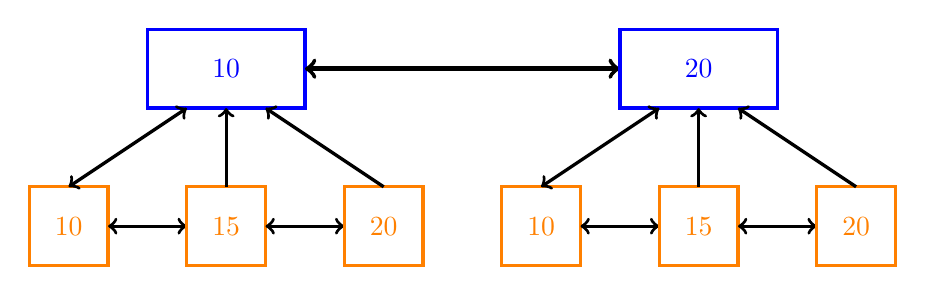
\begin{tikzpicture}
\draw[blue, very thick] (1.5,0) rectangle (3.5,1) node[pos=.5]{10};
\draw[ultra thick, <->] (3.5,0.5) -- (7.5,0.5);
\draw[blue, very thick] (7.5,0) rectangle (9.5,1) node[pos=.5]{20};

\draw[orange, very thick] (0, -2) rectangle (1,-1) node[pos=.5]{10};
\draw[very thick, <->] (0.5,-1) -- (2,0);
\draw[very thick, <->] (1,-1.5) -- (2,-1.5);
\draw[orange, very thick] (2, -2) rectangle (3,-1) node[pos=.5]{15};
\draw[very thick, ->] (2.5,-1) -- (2.5,0);
\draw[very thick, <->] (3,-1.5) -- (4,-1.5);
\draw[orange, very thick] (4, -2) rectangle (5,-1) node[pos=.5]{20};
\draw[very thick, ->] (4.5,-1) -- (3,0);

\draw[orange, very thick] (6, -2) rectangle (7,-1) node[pos=.5]{10};
\draw[very thick, <->] (6.5,-1) -- (8,0);
\draw[very thick, <->] (7,-1.5) -- (8,-1.5);
\draw[orange, very thick] (8,-2) rectangle (9,-1) node[pos=.5]{15};
\draw[very thick, ->] (8.5,-1) -- (8.5,0);
\draw[very thick, <->] (9,-1.5) -- (10,-1.5);
\draw[orange, very thick] (10, -2) rectangle (11,-1) node[pos=.5]{20};
\draw[very thick, ->] (10.5,-1) -- (9,0);

\end{tikzpicture}
\caption{An Order Maintenance data structure. The blue node represent the higher level doubly linked list, and each node store a lower level doubly linked list, denoted by the orange node. Lower level node also store a pointer to the higher level node. Each node additionally hold an unsigned integer, label, such that inside a single list the node earlier have a strictly smaller label then the node later.}
\label{fig:om}
\end{figure}

\subsection{Bulk insertion and deletion}

\label{sec:tree-insertion}
Bulk insertions into the layout tree are common,
  often due to a ``lazy loading'' pattern:
  a ``shell'' web page loads first and shows a loading indicator;
  then the ``content'' loads and is inserted into the page
  as a single large subtree.
This pattern is encouraged by frameworks like React,
  and can occur in several stages, with a ``shell''
  first inserting ``subshells'' which
  themselves load subcomponents in turn.
Efficiently inserting the large subtree
  requires special care in Spineless Traversal.

The basic issue is that all fields of all nodes in the subtree
  need to have them and their OM objects initialized,
  yet we also want subtree insertion to be fast.
Our solution adds these ``initialization passes''
  as special elements in the priority queue.%
\footnote{
  Just enqueueing all fields of all nodes in the subtree
    is not a good idea---it will create a large queue with slow queue operations.
  In our experiments, this often took the queue
    from tens to thousands of members,
    leading to a small integer slowdown.
}
In other words, the priority queue can contain
  not only $(n, v)$ pairs for a dirtied field
  but also $(r, p)$ fields pointing to the root $r$
  of an entire subtree that needs to be initialized
  for pass $p$.
When a subtree $T$ is inserted, each pass for it is enqueued;
  the Order Maintenance object for that
  is created after the OM of the last field
  initialized by $P$ in $T$'s previous sibling or parent.
In this way, we maintain the consistency of incremental layout 
  with from-scratch layout.
\footnote{
  An edge case is inserting a subtree into
    a subtree that itself has not yet been laid out.
  In this case no further actions need to be taken,
    since both subtrees will be visited together.}

When one of these $(r, p)$ elements is popped from the queue,
  the pass $p$ is performed on the whole subtree under $r$,
  creating all necessary order maintenance nodes.
Since all fields in newly-created nodes are initially dirty,
  performing this pass will not enqueue any fields
  in the priority queue,
  meaning that no priority queue operations
  need to be performed.
Likewise, since all data accesses are local,
  no existing nodes will refer to any newly-inserted node
  except the root node,
  so no nodes need to be dirtied when running $p$ on the subtree.
This means that, when initializing a subtree,
  no priority queue operations or dirty bit propagations
  need to be performed,
  which makes subtree insertion faster.
(However, order maintenance objects still need to be created,
  meaning that, despite these optimizations,
  Spineless Traversal is typically
  slower than Double Dirty Bit
  for subtree insertion.)

When deleting a subtree,
  some nodes in the subtree may
  already be in the priority queue;
  for example, this can happen if
  a subtree is inserted and then later deleted.
To avoid unnecessary recomputation,
  we add a ``deleted'' bit to each node
  and skip recomputing such node.%
\footnote{Those nodes are ref-counted and the memory will be reclaimed at the right moment.}
\section{Optimization}
The Double Dirty Bit algorithm uses minimal computation (just set a bit!)
  but is extremely cache-unfriendly (accesses the spine + 1),
  while the spineless traversal is computationally expensive
  (priority queue and order maintenance)
  but cache-friendly (accesses only necessary nodes).
For spineless traversal to be faster,
  the computationally expensive steps in spineless traversal
  have to be meticulously optimization
  to avoid allocation, reduce memory traffic,
  and optimize branch mispredictions.

\subsection{Subtree Insertion}
\label{sec:tree-insertion}
Bulk insertions into the layout tree are common in our data set.
This typically seems to be the result of lazy loading:
  a ``shell'' web page loads first, and shows a loading indicator;
  then the ``content'' loads and is inserted into the page
  as a single large subtree.
This can occur in several stages, with a ``shell''
  first inserting ``subshells'' which in turn load subcomponents themselves.
Handling this requires
  efficient bulk insertion of a large subtree in one step.%
\footnote{
  Just enqueueing all fields of all nodes in the subtree
    is not a good idea---it will create a large queue with slow queue operations.
  In our experiments, this often took the queue
    from tens to thousands of members, leading to a small integer slowdown.
}

Our solution treats inserted subtrees as a single unit in the priority queue.
In other words, queue elements now refer to either a single node
  or to the whole subtree rooted at that node;
  the order maintenance order for either node is the same.
At allocation time, new layout nodes have all their fields dirty;
  thus, a queue cannot contain both a single-node and subtree object
  for the same node.
When a subtree object is dequeued from the priority queue,
  the current layout pass is performed on the whole subtree,
  creating all necessary order maintenance nodes in the correct order.
Throughout this pass, no nodes are enqueued or dequeued
  saving queue traffic and shrinking the size of the queue.
Note that any nodes that refer to the newly-inserted node
  do so through paths like \textsf{prev} or \textsf{first};
  these fields are dirtied when the subtree is inserted
  so do not need to be dirtied again
  when the subtree layout pass is done.

\subsection{Pointer Compression and Custom Allocator}
Order maintenance objects have to be allocated every time
  new layout nodes are inserted;
  optimizing that allocation is essential.
We use a hand-written pool allocator for order maintenance objects;
  in fact, we use separate pools for high- and low-level objects
  to enhance locality.
Since allocations are always for the same size,
  our custom allocator is significantly simpler than the system allocator.

Our pooled allocator, \texttt{OMPool},
  is shown in Figure~\ref{fig:allocator}.
It is paramaterized by \emph{two} types:
  the type of allocated object \texttt{T}
  and the index type \texttt{P} for pointers to allocated objects.
Crucially,
  \texttt{malloc} and \texttt{free} return and consume
  the pointer type \texttt{P} instead of raw pointers.
By making \texttt{P} a smaller integer type,
  like \texttt{uint32} or \texttt{uint16}, this not only saves memory but also increases
  the number of order-maintenance objects per cache line,
  which in turn improves throughput.
In our implementation, we use 32-bit pointers;
  this limits web pages to a few billion elements,
  a size far beyond what any browser can handle,
  but conveniently makes the total size
  of an order maintenance object 128 bits.
Exactly two order maintenance objects
  then fit in each cache line,
  with no order maintenance objects split across two.
By contrast, an experiment with 16-bit pointers
  actually increased runtime---because, we suspect,
  it lead to order maintenance objects
  splitting across two cache lines,
  which introduced additional stalls.

The actual implementation of \texttt{OMPool} is standard;
  it stores a \texttt{pool} of memory as a \texttt{std::vector},
  in which we ensure sufficient capacity at startup.
Freed elements are placed in a separate \texttt{freed} vector,
  which is preferentially drawn from by \texttt{malloc}.
Because the objects are all the same size,
  there is no fragmentation and \texttt{malloc}/\texttt{free}
  are nearly instantaneous.
Moreover, since spineless traversal
  creates order maintenance objects in order,
  allocation patterns are extremely favorable,
  with nearby nodes placed nearby in memory.

\begin{figure}
\begin{verbatim}

template<
  typename T,             // Type of allocated object
  typename P=uint32_t     // Integer type for "pointers"
> struct OMPool {
  std::vector<T> pool;    // Fast allocation, maximize cache usage

  std::vector<P> freed;   // Rapid reuse minimizes cache churn
  
  // Implementation is straightforward
  T* addressof(P p) { return &(pool[p]); }
  P malloc();
  void free(P p) { freed.push_back(p); }
}
\end{verbatim}
\caption{A pooling allocator that focuses on reducing cache misses.}
\label{fig:allocator}
\end{figure}

\subsection{Branchless Order Maintenance Comparison}
Priority queue pushes and pops spend basically all of their time
  comparing order maintenance objects.
Order maintenance objects are small and,
  thanks to our allocator, local in memory,
  making cache misses rare when accessing them.
However, order maintenance object comparison has two cases
  (same or different second-level lists)
  and the bottleneck ends up being the pipeline stall
  induced by the conditional.
The branch predictor does not help much,
  because (thanks to the heap) the comparison is unpredictable.
We therefore implemented a branchless comparison function,
  relying on conditional move instructions instead;
  in a microbenchmark, this reduces comparison time
  to 5 cycles; Figure~\cite{fig:compare} shows the
  assembly implementation.


\begin{figure}
\begin{verbatim}
bool operator<(const _l2_node &l, const _l2_node &r) {
  Label lpl = l.parent->label, rpl = r.parent->label;
  Label ll = l.label, rl = r.label;
  uint64_t result;
  asm volatile(
  
    "xor   %%rbx,  %%rbx    \n"
    "cmp   %1,     %2       \n"
    "seta  %%bl             \n"
    "xor   %%rax,  %%rax    \n"
    "cmp   %3,     %4       \n"
    "seta  %%al             \n"
    "cmove %%rbx,  %%rax    \n"
    
    : "=&a"(result)
    : "r"(ll), "r"(rl), "r"(lpl), "r"(rpl));
  return result;
}
\end{verbatim}
\caption{
  The branchless comparison code is 7 instructions long,
    but the two \texttt{xor} instructions
    clear a register and are thus handled by the register renamer;
    the result is a five-cycle comparison
    for order-maintenance objects.
}
\label{fig:compare}
\end{figure}

\subsection{Dependency Deduplication}

When synthesizing the dirty bit propagation code,
  we make sure to only dirty any given field once per field computation.
For example, if a field $N.V$ is used twice in an expression,
  or if two different paths $\mathsf{first}.V$ and $\mathsf{last}.V$
  reverse to the same field,
  the field is only dirtied once.
This deduplication is especially challenging in the case
  of $N?$ expressions,
  since whether or not a field is dirtied can depend on whether an element
  is the first/last/other child of its parent.
Moreover, the dirty bit is checked before pushing to the priority queue;
  this means a node field only appears in the priority queue once,
  which keeps the queue small.

\subsection{Field packing}

To further shrink the size of the priority queue,
  we use a single dirty bit to cover multiple co-computed fields.
Instead of a dirty bit per field,
  we use two dirty bits per pass---%
  one for the pre-order-computed fields
  and one for post-order-computed fields.
This further reduces the number of unique dirty bits
  set during the dirty bit propagation.
Field packing in this way is a common optimization in real browsers;
  the trade-off is that it reduces the complexity
  (and thus cache misses in) invalidation traversal
  at the cost of possibly more field recomputations
  (since the browser must now recompute \emph{all} covered fields
  when a dirty bit is set)l
  the trade-off appears to be worth it.
The priority queue now likewise store objects
  that name a pass (and a pre/post location)
  instead of a specific field,
  and order maintenance objects likewise correspond
  to passes (plus pre/post) instead of to individual fields.
This reduces the number of OM objects needed
  and reduces the size of the priority queue.
More generally, one can think of the priority queue
  as storing dirty bits themselves,
  however those are assigned by the application in question.
Spineless traversal can thus be applied
  to finer- or coarser-grained field packing,
  though it also benefits more from coarser-grained packing,
  which makes the priority queue smaller and speeds up operations on it.

\subsection{Field representation}

Recall that priority queue entries
  refer to either a subtree or a node,
  and also name a phase plus pre/post location.
We combine the subtree-or-node bit with the phase and pre/post location
  into a simple enum, which we store in a byte.
We use the enum as an index into a jump table,
  while allows us to efficiently execute the field recomputation
  that corresponds to a single priority queue entry.

\subsection{Attempted, Failed Optimizations}

We also attempted a number of further optimizations
  that did not improve performance.
Ultimately, low-level cycle counting is an empirical art,
  and we don't have clear explanations for why these failed.
\begin{itemize}
\item A hybrid between Double Dirty Bit and spineless traversal,
  using a summary bit for subtree dirty bit propagation
  but the priority queue for more distant jumps.
  We were unable to make switching between the two modes efficient enough
  to be competitive.
\item Use a splay tree for the priority queue to improve locality.
  Resulted in a slowdown.
\item Use a red-black tree for the priority queue.
  Resulted in a slowdown. The classic min-heap is best.
\item Use a 1-based array representation for binary heap
  to cut instructions when finding the parent/children.
  Resulted in a slowdown.
\item Cut \texttt{OMPool} pointers to 16 bits, and use 16-bit OM labels.
  Did not see a speedup compared to 32 bits.
\item Pointer tagging to move boolean bit into pointers to reduce object size.
\item Storing the \texttt{left}/\texttt{right} pointers in the OM list in a different location from the elements \texttt{label} and the \texttt{parent}/\texttt{children} pointer, to improve cache locality. Did not see improvement.
\item Deallocating OM objects when the corresponding tree node is deleted, to increase cache locality. Did not see improvement.
\end{itemize}
\section{MegaTron}

To evaluate Spineless Traversal,
  we implement it for a simplified web layout algorithm
  implemented in the DSL of Figure~\ref{fig:dsl}
  and compiled by a compile we call MegaTron.
In this section, we first describe
  the layout modes implemented,
  then how we compile the DSL to a layout engine,
  and finally compare Spinless Traversal to Double Dirty Bit
  on a collection of real-world web page interactions.

\subsection{Web Layout Algorithm}
\label{sec:layout-impl}

To compare Spineless Traversal and Double Dirty Bit,
  we needed a web layout algorithm
  that was decoupled from its invalidation strategy.
Unfortunately, existing browser rendering engines
  are too complex and too tightly coupled
  to their current invalidation strategy,
  making it impossible to reuse them.
We instead implemented our own web layout algorithm
  based on the Cassius and MEDEA formalizations%
  ~\cite{cassius-1,cassius-2,yufeng-2}.
Naturally, this implementation is simplified
  compared to a real-world web browser
  and only implements a subset of features.
However, we took care to implement several features
  with complex invalidation behavior,
  including intrinsic width, flex-box layout, and positioning.
In total, our implementation is 700 lines of code
  in a custom DSL called Megatron,
  which compute approximately 50 fields for each layout node.
The remainder of this section describes
  several key layout features implemented in our layout algorithm.

\paragraph{Box model}.
Each layout node has an $x$, $y$, width and height field.
Typically the rectangle this represents contains
    all of the node's children, while sibling elements
    don't overlap.
In general, width is computed top-down
  (children's width depend on parent's width),
  height is computed bottom-up
  (parent's height is sum of children's heights)
  and $x$ and $y$ are computed in-order.
This forms long dependency chains between elements,
    where updating one element can cause many others
    to be transitively dirtied.
However, the \texttt{width},
    \texttt{min-width}, and \texttt{max-width} CSS properties,
    and similar for \texttt{height},
    can directly set width and height,
    breaking these dependency chains.
Our layout algorithm's support for these properties
    means this early-stopping behavior is tested.
That said, even the
  explicit \texttt{width} and \texttt{height} properties
  allow ``percentage values'' like \texttt{50\%},
  which are resolved relative to the parent and thus
  still create inter-node dependencies.
	
\paragraph{Line Breaking}
Line breaking lays out inline layout nodes (text)
  horizontally from left to right,
  until the edge of the parent box is reached,
  and which point the next layout node is placed
  at the left edge of its parent,
  one line below its previous sibling.
Line breaking requires handling control dependencies,
  where one layout nodes' width may move layout nodes
  from one line to another by changing line breaking.
Additionally, our layout algorithm
  allows different lines to have different height
  (based on the height of the largest layout node in the line),
  which introduces a field (line height)
  that is dependent on may different nodes (each word in the line).
This has a number of interesting effects for invalidation.
For example, adding a node node to a line
  may cause no change if it is not the tallest node in the line.
However, if the new node is now the tallest node,
  that may cause the line to become taller,
  which in turn can cause all other text on the page to move down,
  causing a lot of invalidation.

\paragraph{Display}
Nodes have a \texttt{display} property that changes
  whether they act line words (\texttt{inline})
  or paragraphs (\texttt{block}).
The \texttt{display} property can also be set to \texttt{none},
  in which case the layout nodes are not shown on the page
  and have almost no effect on layout.
Changing a layout node's \texttt{display} property
  between \texttt{block} and \texttt{none}
  is a common way to implement drop-down menus,
  pop-ups, and other elements that appear and disappear,
  such as the ``preview'' hover effects on Wikipedia.
Importantly,
  changes to \texttt{display: none} nodes
  should not invalidate any other nodes and should be fast.
On the other hand, a node switching
  from \texttt{display: none} to \texttt{display: block}
  effectively adds a subtree to the layout tree,
  which is handled specially in Spineless Traversal.
  
\paragraph{Position}
An element with \texttt{position: absolute}
  is manually assigned a position on the page
  by the web developer.
This is commonly used for popups, tooltips, and other effects
  that appear over other page content.
It is also common
  to change the manually-assigned $x$ and $y$ positions
  from JavaScript, such as to move a tooltip away from the cursor.
Layout nodes with absolute positioning do not affect
  the position of other layout nodes outside their subtree,
  and handling changes to $x$ and $y$ positions quickly
  is essential.

\paragraph{Intrinsic sizes}
In a number of cases,
  a layout node's width or height is computed from
  its ``intrinsic'' size,
  which effectively measures how large it would need to be
  to contain all its text without line breaks.
For example, absolutely-positioned elements
  compute their width and height this way by default.
Importantly, intrinsic widths are computed bottom-up,
  but then used in the top-down width computation
  and then the bottom-up height computation.
This means intrinsic sizes require the use of
  multiple layout phases
  and require Spineless Traversal to support such.

\paragraph{Flex-box}
Flex-box layout is the most complex feature
  our layout algorithm supports.
In flex-box layout there is flex container element
  whose children are flex items.
The width/height of flex items depends on
  the intrinsic sizes of the other flex items and
  the actual size of the flex container.
Properties like \texttt{flex-grow} and \texttt{flex-shrink}
  determine how the intrinsic sizes of the flex items
  are adjusted to compensate for either extra or not enough
  available space in the flex container.
The \texttt{max-} and \texttt{min-width}/\texttt{height} properties
  can also cap the growth/shrinkage of individual flex items.
In all, our implementation of flex-box layout
  uses 9 of intermediate fields
  and requires 2 passes to compute all of them.

\paragraph{Miscellaneous}
We also implemented a variety of miscellaneous features,
  including automatic sizing of images and video,
  manual line breaks with the \texttt{<br>} element,
  and conditional elements like \texttt{<noscript>}
  (which are only rendered if JavaScript is disabled,
  not the case in our tests).
We also had to add a special case for \texttt{<svg>} elements,
  whose children describe drawing commands
  that do not participate in layout.
Finally, a variety of minor tweaks
  like the \texttt{width} and \texttt{height} HTML attributes
  (which behave slightly differently from the CSS properties)
  were also implemented.

\subsection{Compiler}
\label{sec-compiler}

\todo{Talk about spineless tagless}

This layout algorithm is implemented in the Megatron DSL
  and then compiled to C++ to maximize performance.
Passes are compiled to three C++ functions:
  the pass itself,
  a function that performs just the pre-order assignments
  and a function that performs just the post-order assignments.
The compiler type-checks all fields, attributes, and properties
  using Hindley-Milner type inference~\cite{HM}
  and uses appropriate unboxed C++ member variables
  to store the relevant values.
Importantly, this means a single node and all its fields
  are contiguous in memory
  (as it would be a real web browser)
  with a minimum of pointers
  (beyond the standard parent/first/last/next/previous pointers
  to other layout nodes)
  and that field access is compiled to a memory offset.
All string values (like the keyword values for \texttt{display})
  are interned and represented in C++ as
  a single \texttt{enum} type,
  meaning that no string allocation or comparison
  is performed at runtime.
Discriminated unions are used for fields with units.
The bottom line is that the compiled code is
  long but readable, idiomatic, and performant C++ code
  with no allocation, hash, or string operations.
This is critical, because it means that,
  like in a real web browser,
  computing fields is very fast
  and the cache misses from finding dirty fields
  are a measurable fraction of the runtime.

The compiler also synthesizes all
  dirty bit propagation code.
Specifically, the compiler examines
  each assignment in each pass,
  determines which fields on which neighbor nodes are read
  to compute each field,
  and computes the inverse neighbor relation.
Every field assignment
  compares the new and old value in the field
  and sets dirty bits only if the new and old value differ.
The actual invalidation traversal algorithm
  (Double Dirty Bit or Spineless)
  is encapsulated in an global value
  that provides a method to dirty a node/field
  and an iterator over all dirty nodes.
The incremental layout entry point function
  iterates over all dirty nodes
  and calls the relevant pass functions.
The compiler also generates functions to modify the tree,
  either by inserting and deleting tree nodes
  or by changing an attribute or property.
These generated functions dirty the appropriate nodes and fields,
  including using the special case for subtree insertion
  for Spineless Traversal.

To ensure our implementation is correct,
  the compiler can also generate a from-scratch layout function
  which does not use dirty bits at all
  and instead recomputes the entire layout from scratch.
This was extremely valuable during development
  and gives us confidence that our invalidation algorithm is correct.

\section{Evaluation}

We use this web layout algorithm
  to compare Spineless Traversal
  against the Double Dirty Bit algorithm
  on \NumWebsites real-world websites.

\subsection{Benchmarks}

To evaluate web layout for these websites,
  we modified the Ladybird web browser
  to dump the layout tree at every rendered frame;
  we then use a separate program to ``diff'' successive frames,
  outputting a list of insertions, deletions,
  and attribute/property changes.
A benchmark program then reads the diff
  and performs each modification in the list,
  then invokes the incremental layout entry point.
Both invalidation and recomputation time
  are measured using the \texttt{rdtsc} instruction,
  allowing a granular comparison of both
  Spineless Traversal and Double Dirty Bit.
In total, the \NumWebsites websites generate traces
  with \NumFrames frames in total.
Each frame leads to a single incremental layout call,
  so our experiment has \NumFrames individual data points.
Note that this large number of frames,
  covering gigabytes of layout tree data,
  nonetheless represents only a few minutes of web browsing activity.
All experiments are run on a machine with
  an Intel i7-8700K CPU (8th generation)
  clocked at the standard 3.70\,GHz
  with 64\,KB L1 cache, 256\,KB L2 cache (both per core),
  and 12\,MB L3 cache, plus
  32\,GB of DDR4 memory across 4 DIMMs,
  each configured to 3000 MT/s.

The \NumWebsites real-world websites include
  Amazon, Wikipedia, Github, Google,
  as well as a number of other popular websites
  drawn from the Alexa ranking of top websites
  and focusing on large web pages and complex web applications.
It also includes a number of personal favorites of the authors,
  including Github and Lichess.
We focus on latency-sensitive interactions
  like hovering, typing, dragging, and animations.
These interactions typically
  do not require loading data over the network
  and invalidation time is thus a big determinant of their latency.
By contrast, interactions like loading a whole web page
  or moving between portions of a website
  typically have network latency which far overshadows
  any possible invalidation latency.
Even though the interactions may seem minor,
  it is important to note that the browser is nonetheless
  performing a significant amount of work to render them.
For example, on Wikipedia, hovering over a link
  shows a ``preview'' window,
  and Wikipedia code must track and respond to mouse movements
  to hide and show the preview window at the correct time.
Moreover, there is a short, nearly-imperceptible animation
  by which the preview window slides and fades in and out of view.
Similarly, on the Lichess web page,
  our trace captures one of the authors
  stepping through a chess opening using the website's
  chess commentary tools.
The Lichess website renders the chess board using HTML elements
  and each move animates visual aids like arrows.
Text editing, an especially latency-sensitive interaction,
  was also tested.
For example, on the Google website we tested
  typing a search term letter by letter,
  with the Google website changing autocomplete suggestions
  as we typed.

\subsection{Results}

\begin{figure}
\begin{minipage}[t]{0.48\linewidth}
\includegraphics[width=\linewidth]{DBPQOverhead.jpg}
\caption{
The invalidation traversal time for all \NumFrames frames,
    with Double Dirty Bit time on the $x$ axis
    and Spineless Traversal time on $y$ axis.
The diagonal line shows the $x = y$ equal time line;
    points below the line are faster with Spineless Traversal
    while points above the line are faster with Double Dirty Bit.
Both axes are in log scale, meaning Spineless Traversal is often
    tens or hundreds of times faster than Double Dirty Bit.
}
\label{fig:xy}
\end{minipage}\hfill%
\begin{minipage}[t]{0.48\linewidth}
\includegraphics[width=\linewidth]{DBPQCDF.jpg}
\caption{
  A CDF of the ratio between
    Double Dirty Bit time and Spineless Traversal time
    for each frame.
  The vertical line, at $10^0$,
    marks where both invalidation algorithms take equal time.
  To the left of the line,
    \PctSlower of frames are slower with Spineless Traversal.
  To the right of the line,
    \PctFaster of frames are faster with Spineless Traversal.
  The geometric mean speedup with Spineless Traversal
    is \MeanSpeedup.}
\label{fig:cdf}
\end{minipage}
\end{figure}

\iffalse
\begin{figure}
\begin{subfigure}{0.5\linewidth}
    \includegraphics[width=\linewidth]{DBPQLargeOverhead.jpg}
\end{subfigure}\hfill%
\begin{subfigure}{0.5\linewidth}
    \includegraphics[width=\linewidth]{DBPQLargeCDF.jpg}
\end{subfigure}
\caption{
The overhead scatter plot and the speedup cdf,
  restricted to frames where more than 1\% of fields
  are recomputed. These points typically represent loading of new contents.}
\label{fig:dbpq-large}
\end{figure}
\fi

Figure~\ref{fig:xy}
  shows our results.
In Figure~\ref{fig:xy}, points below the diagonal line
  are faster with Spineless Traversal,
  while points above the diagonal line
  are faster with Double Dirty Bit.
Most points are below the line,
  often with enormous speedups: 10--$100\times$.
These points are often interactions
  where only a few deeply-nested nodes are dirtied,
  where Double Dirty Bit accesses a huge number
  of auxiliary nodes.
By contrast, while some points are above the line,
  meaning they are slower with Spineless Traversal,
  they are typically much closer to the line,
  indicating that slowdowns are not as severe
  as the speedups are beneficial.
The geometric mean is a \MeanSpeedup speedup
  from Spineless Traversal,
  with only \PctSlower of frames rendered slower.
Figure~\ref{fig:cdf} shows CDF of the speedup
  of Spineless Traversal over Double Dirty Bit.

Figures~\ref{fig:xy} and~\ref{fig:cdf} show
  only invalidation time,
  including traversal, dirty bit propagation,
  enqueuing nodes in the priority queue (for Spineless Traversal)
  and setting summary bits (for Double Dirty Bit).
We measured field computation time separately,
  and confirmed that it was nearly identical
  between Spineless Traversal and Double Dirty Bit,
  which is as expected since both algorithms will
  recompute the exact same fields in the exact same order.
In total, invalidation time was roughly one third of total runtime,
  while field computation time was roughly two thirds,
  showing that invalidation is a determinant of latency.

A more careful inspection of Figure~\ref{fig:xy} shows
  several additional features.
The slowest frames all feature slowdowns.
This is expected: the slowest frames likely represent
  the initial page load or other ``loading'' frames,
  which we necessarily capture in our traces.
While speedups are always better than slow-downs,
  these loading frames likely follow network latency,
  so invalidation time for these frames is less important.
Meanwhile, frames where fewer nodes are invalidated
  are typically those triggered in response to
  an animation or user interaction,
  where latency is most critical.
Figure~\ref{fig:dbpq-small} shows an analog of
  Figures~\ref{fig:xy} and~\ref{fig:cdf}
  but restricted to points where fewer than 1\% of fields
  are recomputed;
  the intention is that a loading frame typically changes
  large portions of the web page
  while interactions typically change much less.
On this latency-critical subset,
  which contains more than half of frames,
  the geometric mean speedup is larger,
  at \MeanSpeedupSmall,
  and a smaller fraction of frames suffer slowdowns.
Spineless Traversal is also faster on average outside this subset,
  likely because the 1\% threshold is an imprecise heuristic,
  but the dramatically larger speedup in this latency-critical subset
  supports the idea that Spineless Traversal helps most
  precisely on those points where latency is most important.

\begin{figure}
\begin{subfigure}{0.5\linewidth}
    \includegraphics[width=\linewidth]{DBPQSmallOverhead.jpg}
\end{subfigure}\hfill%
\begin{subfigure}{0.5\linewidth}
    \includegraphics[width=\linewidth]{DBPQSmallCDF.jpg}
\end{subfigure}
\caption{The overhead scatter plot and the speedup CDF,
  restricted to frames where fewer than 1\% of fields
  are recomputed.
  These frames typically represent the latency-sensitive
  interactions like hovering, animations or editing.}
\label{fig:dbpq-small}
\end{figure}

\subsection{Case Study: Wikipedia}
\section{Related Work}
Incremental Evaluation of interactive programs have yield a long line of fruitful research, dating back to the 1980s (\citet{TR}), and including work such as \cite{yufeng-2}, \cite{SAC}. OTOH, the industry had developed their own solution, the Double Dirty Bit algorithm, to fulfill their latency need.
\section{Conclusion}
%\bibliographystyle{acm}
\bibliographystyle{ACM-Reference-Format}
\bibliography{main}
\end{document}
